\documentclass[fontsize=12pt,a4paper]{scrartcl}
 
% Das Prozent\item Zeichen leitet einen Kommentar ein,
% es hilft ebenso, im Text Leerzeichen zu unterbinden.
 
% fontsize=12pt  Schriftgroesse in 10, 11 oder 12 Punkt
% a4paper        Papierformat ist hier A4
% landscape      Querformat wird natürlich unterstützt ;\item )
% parskip        Absatzabstand anstatt Einzüge
% draft          Der Entwurfsmodus deckt Schwächen auf
% {scrartcl}     Die Dokumentenklasse book, report, article
%                oder fürs deutsche scrbook, scrreprt, scrartcl
 
%\usepackage[ngerman]{babel} % Deutsche Sprachanpassungen
\usepackage[T1]{fontenc}    % Silbentrennung bei Sonderzeichen
\usepackage[latin1]{inputenc} % Direkte Angabe von Umlauten im Dokument.
                            % Wenn Sie an einem Mac sitzen,verwenden
                            % Sie ggf. „macce“ anstatt „utf8“.
 
\usepackage{textcomp}       % Zusätzliche Symbolzeichen
\usepackage{siunitx}
\usepackage{amsmath}
\usepackage{graphicx}
\usepackage{listings}
\usepackage{float}
\lstset{tabsize=4, showspaces=false}


\title{Machine Learning SS2013}
\subtitle{Ulrike von Luxburg \\ Assignment 10}
\author{Arne Schr�der \and Falk Oswald \and Angel Bakardzhiev}
 
\date{\today}               % \today setzt das heutige Datum
 
\begin{document}
\maketitle                  % Titelei erzeugen
% \tableofcontents            % Inhaltsverzeichnis anlegen

\section*{Exercise 1: Data processing chain}

We used KNime as data processing workflow application.
It works pretty goot and is intuitive to operate. One downside, however, is that you can not easily display numerical loss but have to estimate the resulitng error values. Thus we present graphical results in the sections below.

\subsection*{Regression}
We performed regression on the cancer dataset.
We compared linear regression with polynomial regression. Both seem to work pretty well, as they have both only a few miss-classifications.

    \begin{figure}[H]
        \centering
        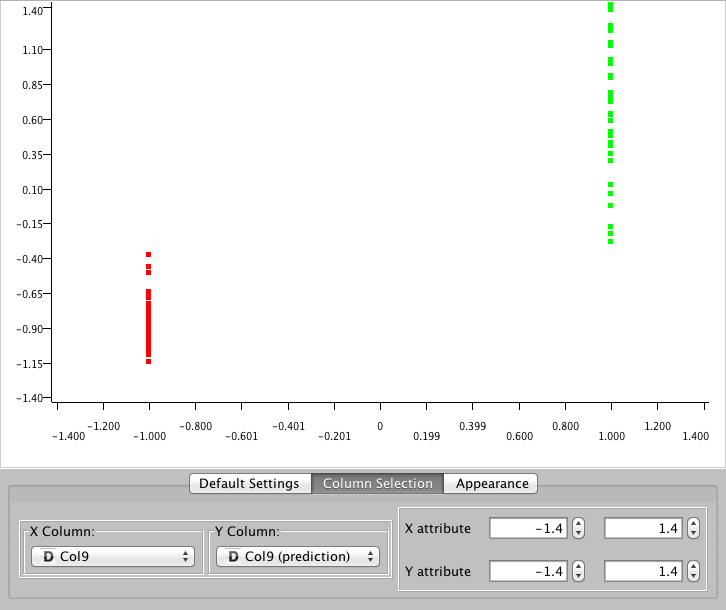
\includegraphics[width=0.9\textwidth]{reg_lin_cancer.PNG}
        \caption{Linear regression result. Y axis are the prediction results, X axis the labels.}
    \end{figure}

    \begin{figure}[H]
        \centering
        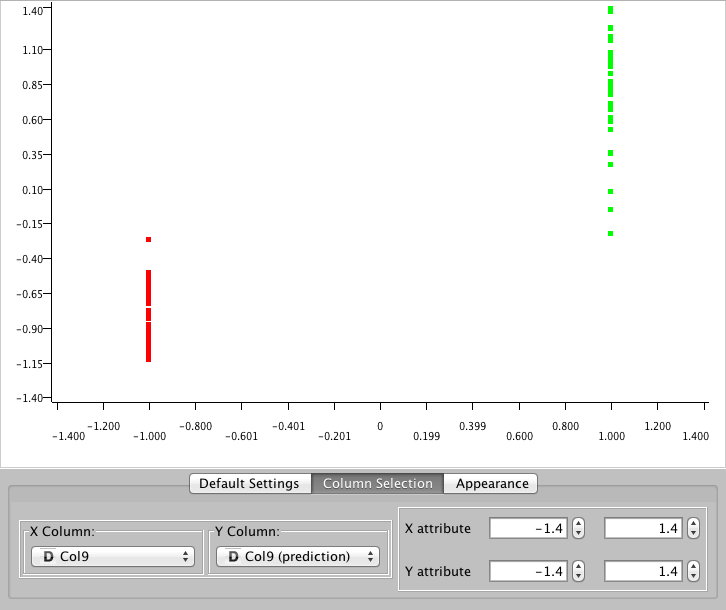
\includegraphics[width=0.9\textwidth]{reg_poly_cancer.PNG}
        \caption{Polynomial regression result. Y axis are the prediction results, X axis the labels.}
    \end{figure}
    
However, the polynomial regression (with degree 2) works slighty better as there are even less missclassifications.	
    
\pagebreak
\subsection*{Clustering}
The Yeast dataset seems pretty hard to cluster. kMeans as well as hierarchical clustering do not perform well at all. Howeve, if you use PCA for dimensionality reduction, the clustering looks much better.

\subsubsection*{Yeast Clustering without PCA}
    \begin{figure}[H]
        \centering
        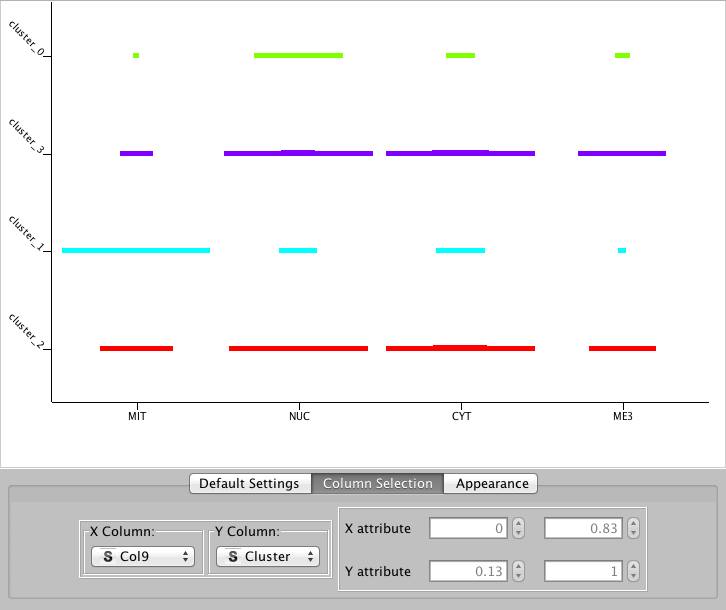
\includegraphics[width=0.9\textwidth]{cluster_kMeans_yeast.PNG}
        \caption{Clustering of the yeast dataset fails nearly completely. The figure shows that all classes overlap quite a lot. At least cluster 0 and cluster 1 have one mayor label representation (cluster 0 = NUC, cluster 1 = MIT)}
    \end{figure}

    \begin{figure}[H]
        \centering
        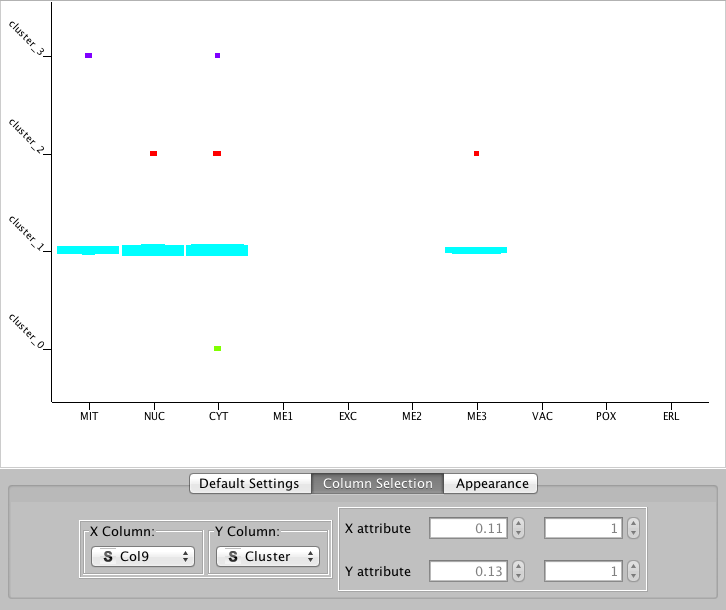
\includegraphics[width=0.9\textwidth]{cluster_hierarchical_yeast.PNG}
        \caption{Hierarchical clustering works even worse. Nearly all data are classified into one cluster}
    \end{figure}

\subsubsection*{Yeast Clustering with PCA}
    \begin{figure}[H]
        \centering
        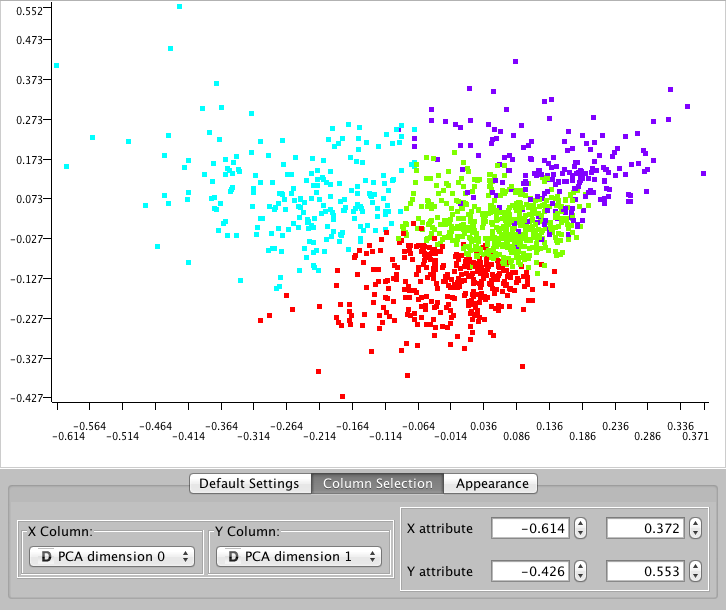
\includegraphics[width=0.9\textwidth]{cluster_kMeans_yeast_PCA.PNG}
        \caption{kMeans with PCA produces a much better result as cluster blobs can easily be recognized}
    \end{figure}

    \begin{figure}[H]
        \centering
        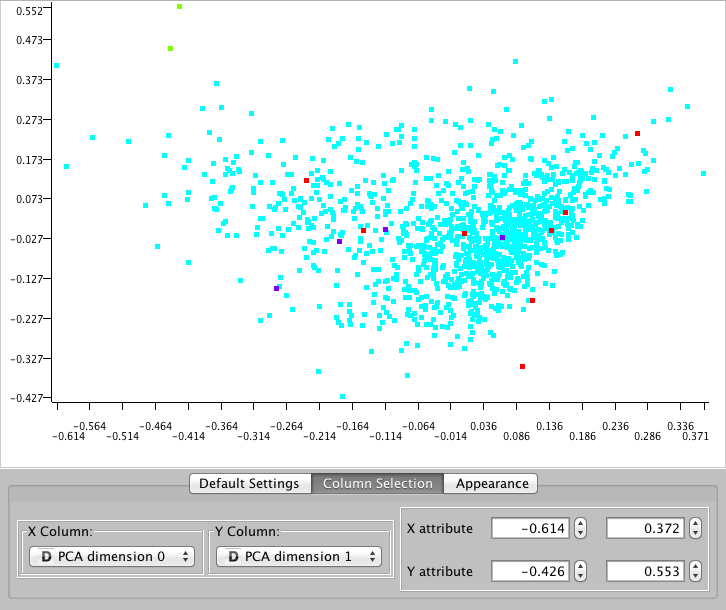
\includegraphics[width=0.9\textwidth]{cluster_hierarchical_yeast_PCA.PNG}
        \caption{As opposed to kMeans/PCA, hierarchical clustering still does not work at all with PCA.}
    \end{figure}


\subsubsection*{Synthetic data Clustering without PCA}
We used the kNime synthetic data generator to create a synthetic dataset.
The created data constisted of 4 clusters with noise as displayed in the figure below.
    \begin{figure}[H]
        \centering
        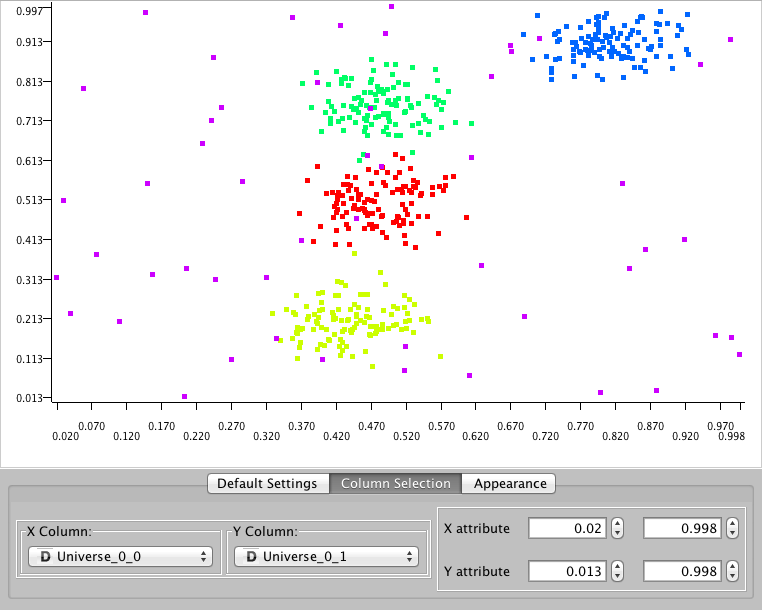
\includegraphics[width=0.9\textwidth]{cluster_synthetic_data.PNG}
        \caption{KMeans clustering of synthetic data}
    \end{figure}
    
    \begin{figure}[H]
        \centering
        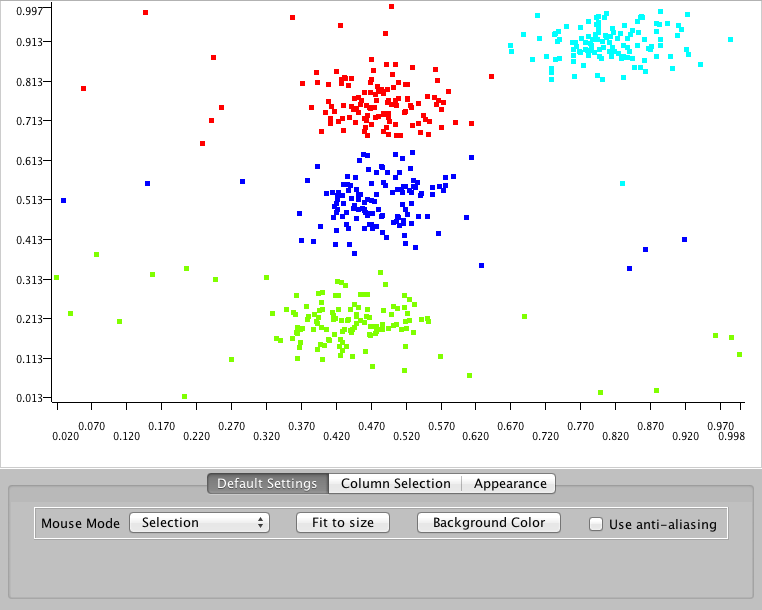
\includegraphics[width=0.9\textwidth]{cluster_kMeans_synthetic.PNG}
        \caption{KMeans clustering of synthetic data}
    \end{figure}
    
    \begin{figure}[H]
        \centering
        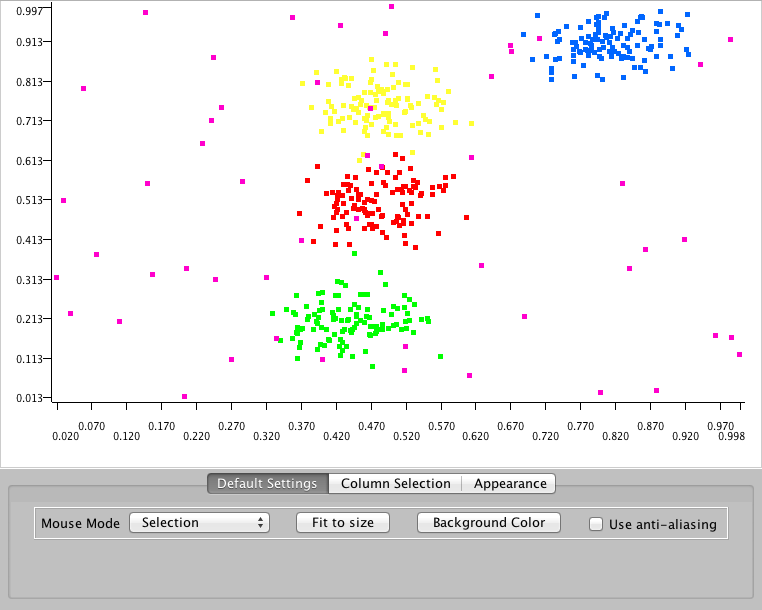
\includegraphics[width=0.9\textwidth]{cluster_hierarchical_synthetic.PNG}
        \caption{Hierarchical clustering of synthetic data}
    \end{figure}
    
    As expected, the clustering on this gaussian distributed clusters works pretty good.
    However, as kMeans only detects the clusters and assigns the "nearest noise" to the clusters, hierarchical clustering even detects the noise data appropriately.
    
\end{document}